\begin{reviewcallout}\textbf{Reading boundary}\\Literature search cutoff: 29 October 2026; targeted follow-up verification: 2 November 2026. Published findings, our historical pilot and proposed research are distinguished throughout. Prepared for the November supervisor discussion.\end{reviewcallout}

\begin{abstract}

Communication compression in federated learning changes both the representation of an update and, potentially, the optimization trajectory. This review connects the main research lines: stochastic quantization, coordinate sparsification, error feedback, low-rank approximation, learned representations and source coding. It compares what is transmitted, the conditions behind error or convergence claims, and costs often hidden by nominal compression ratios. Adaptive methods already change precision across rounds and clients, exploit side information, or choose among compression strategies. Accordingly, an adaptive Lempel-Ziv contribution must be positioned more narrowly than the general idea of adaptive compression.

The thesis investigates second-stage LLZ tolerance selection after a fixed QSGD draw. A local reconstruction constraint makes candidate selection testable, but does not establish a learning-safe distortion budget. A separate DigiFace pilot illustrates the distinction: the tighter adaptive policy reduced training-upload bytes relative to lossless LLZ while retaining a similar selected validation accuracy in one seed, yet the change in total serialized communication was much smaller. The review identifies budget justification, feedback policy, computational overhead and confirmation evidence as the next methodological priorities. It makes no priority, statistical-equivalence or new convergence claim.

\end{abstract}

\tableofcontents\clearpage
\pagenumbering{arabic}
\setcounter{page}{1}

\section{FL updates and communication accounting}

Federated averaging allows clients to perform local training before the server combines their model updates. A transmitted local model difference is therefore a closer abstraction for this project than a single gradient evaluated at the broadcast model. The distinction matters when using theory from distributed SGD: an unbiased codec preserves its input in conditional expectation, but does not turn a multi-step local trajectory into an unbiased gradient at the global iterate. \parencite{mcmahan2017fedavg,wang2021fieldguide}

\begin{figure}[htbp]\centering
\begin{tikzpicture}[node distance=8mm and 7mm]
\node[reviewbox] (s1) {Server\\broadcast $w_t$};
\node[reviewbox,right=of s1] (c) {Client $i$\\$H$ local steps};
\node[reviewbox,right=of c] (enc) {Encode/decode\\delta $u_{i,t}$};
\node[reviewbox,right=of enc] (s2) {Server\\weighted update};
\draw[reviewarrow] (s1)--(c);\draw[reviewarrow] (c)--(enc);\draw[reviewarrow] (enc)--(s2);
\node[below=4mm of c,text=Ink,font=\footnotesize] {Repeated for sampled clients; preserve the local-delta sign and units.};
\end{tikzpicture}
\caption{Local training and compressed model-delta aggregation. Original schematic based on FedAvg; mathematical setting is defined in the text.}
\label{fig:fl}
\end{figure}

Let w\_t be the broadcast model, u\_i,t = w\_i,t,H - w\_t the local delta after H steps, and a\_i nonnegative aggregation weights summing to one. With decoded compressor C, the project uses:

\begin{equation*}w_{t+1} = w_t + \sum_i a_i C(u_{i,t})\end{equation*}

The local learning rate is already included in u\_i,t. Multiplying the decoded delta by that rate again would change the algorithm. Common FL challenges include heterogeneous data, participation and device resources; compression interacts with all three. A communication-efficient representation also does not, by itself, give a formal privacy guarantee. \parencite{kairouz2021advances}

\begin{table}[htbp]
\centering
\small
\begin{tabularx}{\textwidth}{R{0.60000}R{1.40000}}
\toprule
\textbf{Boundary} & \textbf{What is counted} \\\midrule
Codec packet & Compressed content plus codec header, shape and padding. \\
\rowcolor{TableAlt}
Serialized Flower object & Codec plus records, metadata, routing and diagnostics. \\
Whole experiment ledger & All declared uploads, downloads and evaluation exchanges. \\
\rowcolor{TableAlt}
Physical network / energy & Requires transport/device measurement; absent from this pilot. \\
\bottomrule
\end{tabularx}
\caption{Communication boundaries used throughout this review; each saving needs its stated boundary.}
\label{tab:accounting}
\end{table}

This review treats setup and decoder distribution as actual transfers when required. Local state and rejected-candidate computations consume memory or time even when they are not transmitted. Byte savings must use the same numerator and denominator across a comparison. Our pilot measures serialized Flower objects, including metadata and diagnostics; it does not measure network packets, transport headers or radio energy.

\section{Quantization: numerical operators and encodings}

QSGD stochastically rounds normalized coordinate magnitudes to a finite set of levels while retaining signs and a vector norm. In ideal arithmetic it is conditionally unbiased. For dimension d and resolution s, its relative second-moment error is bounded by the smaller of d/s\textasciicircum{}2 and sqrt(d)/s. This is an expectation bound over quantization randomness, not a hard limit on each encoded update. The original work also supplies a source code for the resulting symbols; quantization and bitstream construction are separate operations. \parencite{alistarh2017qsgd}

\begin{equation*}\mathbb{E}[Q_s(x)\mid x] = x\end{equation*}

\begin{equation*}\mathbb{E}[\|Q_s(x)-x\|_2^2\mid x] \leq \min(d/s^2,\sqrt{d}/s)\|x\|_2^2\end{equation*}

Our QSGD baseline uses a project-defined dense code, rather than the original sparse/Elias-style representation. At levels=127, each coordinate occupies one sign bit and seven magnitude bits. A flat tensor of 4,096 float32 values occupies 4,116 packet bytes including its header and shape, compared with 16,384 raw bytes. Small tensors can expand because metadata is not free. Norms are per tensor, so a bound or cost based on one whole-model normalization would describe a different protocol.

signSGD keeps signs and uses sign-based updates, including majority aggregation in its distributed form. It discards magnitude and changes the optimization procedure. Its results require their own smoothness and gradient-noise assumptions; improved worker scaling adds restrictions on noise. It is not QSGD at one level, because QSGD can also output zeros and retains a norm. \parencite{bernstein2018signsgd}

FedPAQ is a more direct FL bridge: it quantizes model differences after local steps and combines periodic averaging with partial participation. Its analysis uses an unbiased relative-variance quantizer, common IID client data and prescribed optimization conditions. Positive-p LLZ selection has not been shown to satisfy those hypotheses. \parencite{reisizadeh2020fedpaq}

\begin{table}[htbp]
\centering
\small
\begin{tabularx}{\textwidth}{R{0.57000}R{0.96000}R{1.47000}}
\toprule
\textbf{Method} & \textbf{Numerical object} & \textbf{Key limitation} \\\midrule
QSGD & Stochastic levels and norm & Expected error; representation must be specified. \parencite{alistarh2017qsgd} \\
\rowcolor{TableAlt}
signSGD & Signs / majority update & Changes the optimization rule. \parencite{bernstein2018signsgd} \\
FedPAQ & Quantized local differences & IID/unbiased-compressor theory is conditional. \parencite{reisizadeh2020fedpaq} \\
\bottomrule
\end{tabularx}
\caption{Quantization-related methods and why their guarantees are not interchangeable.}
\label{tab:quantization}
\end{table}

The practical implication is to report both the numerical reconstruction rule and the actual coding format. Equal nominal levels do not guarantee equal transmitted bytes. Conversely, lossless recoding of the same quantized symbols can save bytes without changing their reconstruction.

\section{Sparsification, coordinate sets and error feedback}

A coordinate-set compressor retains selected entries and conveys their positions. The supervisor's term L-Set is interpreted here as this family of representations, rather than a uniquely identified named algorithm. Top-k selects the largest magnitudes. Uniform Rand-k selects k coordinates without replacement; leaving them unscaled is biased, whereas scaling retained entries by d/k makes the operator unbiased at the cost of higher variance. \parencite{stich2018memory}

\begin{equation*}\|x-\operatorname{Top}_k(x)\|_2^2 \leq (1-k/d)\|x\|_2^2\end{equation*}

\begin{equation*}\mathbb{E}[\|(d/k)\operatorname{Rand}_k(x)-x\|_2^2] = (d/k-1)\|x\|_2^2\end{equation*}

These fixed-vector identities do not rank multi-round FL accuracy. They also do not remove coordinate-index costs. A sparse message can coexist with dense working memory, optimizer state and a dense residual.

Error feedback compensates unsent information in a later update. The mechanism is distinct from the compressor: add the residual, compress and locally reconstruct, then store the difference. The project uses the following delta-space bookkeeping for Top-k:

\begin{figure}[htbp]\centering
\begin{tikzpicture}[node distance=8mm and 7mm]
\node[reviewbox] (a) {Correct input\\$v=u+e$};
\node[reviewbox,right=of a] (b) {Codec + decode\\$c=C(v)$};
\node[reviewbox,right=of b] (c) {Store residual\\$e_{\mathrm{next}}=v-c$};
\draw[reviewarrow] (a)--(b);\draw[reviewarrow] (b)--(c);
\draw[reviewarrow] (c.south) -- ++(0,-7mm) -| (a.south);
\node[below=12mm of b,text=Ink,font=\footnotesize] {Residual retained locally for the next client update};
\end{tikzpicture}
\caption{Error feedback in model-delta units. Original schematic; residuals refer to the complete decoded compressor.}
\label{fig:ef}
\end{figure}

\begin{equation*}v_{i,t}=u_{i,t}+e_{i,t};\qquad c_{i,t}=\operatorname{decode}(\operatorname{encode}(v_{i,t}))\end{equation*}

\begin{equation*}e_{i,t+1}=v_{i,t}-c_{i,t}\end{equation*}

Memory/EF results are conditional on the optimization and compressor assumptions in the respective papers. They do not certify every byte codec or arbitrary local-epoch implementation. Residuals must have consistent units and persist with the correct client and run lineage. A model checkpoint alone cannot resume them. \parencite{stich2018memory,karimireddy2019error}

For a future QSGD-plus-LLZ feedback variant, residuals would need to account for the complete decoded composed compressor. Correcting only extra LLZ error leaves QSGD error uncompensated. The current QSGD/LLZ/adaptive pilot has no EF, whereas the earlier Top-k baseline uses EF. Those earlier comparisons cannot isolate compressor choice from feedback policy.

\section{Practical sparse systems and low-rank compression}

Deep Gradient Compression combines sparsification with momentum correction, local clipping, momentum-factor masking and warm-up. Its contribution is the system of these mechanisms, not simply retaining the largest entries. Its encoding and empirical performance belong to that complete design. Calling the project's Top-k-plus-EF baseline DGC would therefore overstate what was implemented. \parencite{lin2018dgc}

PowerSGD exploits matrix structure by communicating low-rank factors. Its power/subspace iteration avoids a full SVD, but the result is not necessarily the exact best rank-r approximation. Residuals, orthogonalization, warm starts and dependent collective communication are important practical components. The original data-parallel method is not reproduced by independently factorizing client matrices and averaging arbitrary factors: averaging products generally differs from multiplying averages. \parencite{vogels2019powersgd}

\begin{table}[htbp]
\centering
\small
\begin{tabularx}{\textwidth}{R{0.75000}R{1.29000}R{0.96000}}
\toprule
\textbf{Representation} & \textbf{Declared content / packet cost} & \textbf{Important omission} \\\midrule
Dense FP32 & 32d bits & Protocol framing \\
\rowcolor{TableAlt}
k coordinates & k(32 + ceil(log2 d)) bits & Padding / synchronization \\
Project Top-k & 12 + 8k bytes & Flower layout/state records \\
\rowcolor{TableAlt}
Rank-r n by m factors & 32r(n+m) bits & Other tensors / collectives \\
Project example: d=4096, k=64 & Top-k 524 bytes; dense 16,384 bytes & Not a learning benchmark \\
\bottomrule
\end{tabularx}
\caption{Illustrative accounting; formats and numerical units are explicit. Sparse and low-rank context: \parencite{stich2018memory,vogels2019powersgd}.}
\label{tab:costs}
\end{table}

Table values describe declared logical content or current project packets. Generic coordinate indices use minimally packed fixed-width positions; the project deliberately uses uint32. Generic factor sizes omit uncompressed vector parameters, framing, synchronization and collective-topology costs. A 512 by 512 rank-one example contains 1,024 factor values instead of 262,144 dense values: a 1/256 content ratio before those other costs. This is arithmetic, not an observed training speedup.

The distinction between a compressor and its deployment is central to fair FL comparison. The same nominal sparsity or rank can have different bytes and runtime under different representations. Error feedback may increase local memory without increasing uploads, while decoder/state refresh can add real communication. Our literature coverage includes Rand-k, DGC and PowerSGD, but these are not implemented comparators in the current project.

\begin{reviewcallout}\textbf{Comparison rule}\\Match the training protocol and disclose feedback/state. Compare actual bytes, learning quality and computation together; do not infer bandwidth or energy from an array-size ratio alone.\end{reviewcallout}

\section{Learned compression and decoder costs}

Learned update compression fits an encoder to produce a compact representation and gives the server a corresponding decoder. Chandar and colleagues propose collecting task-model weight trajectories, training client-specific autoencoders and transferring decoder models. Their reconstruction and classifier evidence establishes a prior application of learned coding to FL, but does not give a general convergence guarantee or our matched closed-loop FL benchmark. A nominal latent-dimensional ratio omits decoder distribution and training costs. \parencite{chandar2021autoencoder}

\begin{figure}[htbp]\centering
\begin{tikzpicture}[node distance=8mm and 7mm]
\node[reviewbox] (a) {Client encoder\\local calibration};
\node[reviewbox,right=of a] (b) {Latent payload\\declared precision};
\node[reviewbox,right=of b] (c) {Server decoder\\synchronized version};
\draw[reviewarrow] (a)--(b);\draw[reviewarrow] (b)--(c);
\node[below=4mm of b,text=Ink,font=\footnotesize] {Decoder distribution and later refresh are additional transfers.};
\end{tikzpicture}
\caption{Learned update coding and the decoder dependency. Original schematic inspired by the AE literature; no learned-codec FL run is claimed.}
\label{fig:learned}
\end{figure}

A deployment must agree on decoder weights and version, tensor layout, normalization and latent representation. Floating-point latent coordinates are not entropy-coded merely because their encoder is learned. Calibration and fitting can be local computation; data transferred for calibration, decoder distribution and subsequent refresh must be counted when they occur. Distribution drift can make an initially effective encoder expensive to maintain or inaccurate later in training.

The project's standalone AE used blocks of 256 coordinates and a six-value latent representation. Its saved-update assessment found smaller constructed bundles than Top-k without feedback, but substantially worse reconstruction. The projection including four decoder artifacts saved 6.42\% of codec-only bytes across 60 uploads. This justified retaining the implementation as offline feasibility evidence rather than integrating it into Flower. It does not establish the general inferiority of learned compressors.

\begin{table}[htbp]
\centering
\small
\begin{tabularx}{\textwidth}{R{1.44000}R{0.78000}R{0.78000}}
\toprule
\textbf{Offline quantity} & \textbf{Block AE} & \textbf{Top-k, no EF} \\\midrule
Constructed bytes / update & 924,310 & 992,594 \\
\rowcolor{TableAlt}
Pooled relative squared error & 0.665316 & 0.264914 \\
Mean full-update cosine & 0.585770 & 0.861918 \\
\rowcolor{TableAlt}
Projected 60 uploads + decoder setup & 55,732,156 bytes & 59,555,640 bytes \\
\bottomrule
\end{tabularx}
\caption{Existing 6 October offline assessment, not a new run. Four AE decoder artifacts total 273,556 bytes; projection excludes Flower/downlink/control traffic.}
\label{tab:ae}
\end{table}

These are historical probe results, not FL identification accuracies. Reconstruction validation selected checkpoints; the trajectories shared the training-image population. They do not evaluate an untouched test set or late-round drift. Timings in the saved decision used a fixed method order and are not randomized throughput measurements.

Recent NNCodec FL work also illustrates a terminology boundary: an encoder/decoder for neural-network parameters need not be an autoencoder latent model. The inspected two-page poster combines update reduction, quantization and DeepCABAC arithmetic coding, with syntax for referencing earlier parameter versions. Its task-specific evidence cannot be transferred to our face-classification protocol. \parencite{becking2025tinyfl}

\section{LLZ-p: source coding after quantization}

LLZ applies dictionary coding to already quantized symbols. The conference predecessor and the 2026 journal article develop lossy Lempel-Ziv compression for FL gradients; the journal also studies side information and hybrids. The accepted Early Access author version is used here, with the earlier supplied manuscript kept as historical implementation provenance. \parencite{zhong2023llz,cao2026llz}

The project parser searches reconstructed history for an approximate match, emits a position/length/following-literal triplet and reconstructs from the same history. It forbids overlapping references and reserves a literal for each phrase. Integer p controls the allowed coordinate-wise symbol mismatch. At p=0, this second stage is lossless relative to the quantized symbols; it does not recover information discarded by QSGD.

\begin{table}[htbp]
\centering
\small
\begin{tabularx}{\textwidth}{R{0.42000}R{1.68000}R{0.90000}}
\toprule
\textbf{Tolerance} & \textbf{Triplets: (position, length, literal)} & \textbf{Decoded symbols} \\\midrule
p=0 & (0, 0, 2); (0, 0, 0); (1, 2, 3); (0, 0, 1); (3, 1, 0) & 2 0 2 0 3 1 2 0 \\
\rowcolor{TableAlt}
p=1 & (0, 0, 2); (0, 0, 0); (1, 2, 3); (4, 2, 0) & 2 0 2 0 3 0 3 0 \\
\bottomrule
\end{tabularx}
\caption{Original worked example: source [2, 0, 2, 0, 3, 1, 2, 0], alphabet bound 3 and window 8. Exact tuples come from the current project parser; packet sizes are deliberately not used to claim compression on this tiny vector.}
\label{tab:llz-example}
\end{table}

The worked example is generated from the current parser, not copied from a publisher figure. Positions are one-based within the available window; position zero denotes a literal-only phrase. The decoded sequence, rather than the original sequence, forms the subsequent dictionary. p is a symbol tolerance, not a percentage or a learning-loss budget. The journal's quantizer uses s-1 intervals, so its s=128 corresponds to our levels=127.

The journal bounds added dequantized error using the mismatch count and the quantization step scaled by p. Its convergence discussion is conditional on the stated stochastic-gradient, smoothness and distortion conditions; it does not show that every fixed positive p preserves convergence. LLZ-SI is an empirical extension outside that theorem. Our local-epoch FedAvg deltas and adaptive selection need separate analysis. \parencite{cao2026llz}

The paper's retained-bit fraction rho uses compressor bits relative to raw FP32 gradient bits, including compressor metadata. Our complete serialized Flower ledger additionally includes downloads and evaluation exchanges. The paper's Table IV concerns PowerSGD-LLZ sensitivity, not QSGD-LLZ; its Table V studies EF. A DigiFace adaptation should not be labeled a numerical reproduction of those CIFAR results.

\section{Adaptation and side information}

Adaptive compression can change representation precision, distribute resources across clients, exploit decoder knowledge, or choose a compressor. These are different control problems and do not share one universal distortion threshold.

\begin{table}[htbp]
\centering
\small
\begin{tabularx}{\textwidth}{R{0.69000}R{1.41000}R{0.90000}}
\toprule
\textbf{Method} & \textbf{Control / objective} & \textbf{Shared or local state} \\\midrule
AdaQuantFL & Precision across training; bound/bit budget & Loss / initial precision \\
\rowcolor{TableAlt}
DAdaQuant & Time/client levels; variance proxy & Loss history / weights \\
KLMS & Side-information sample coding & Distributions / seeds / blocks \\
\rowcolor{TableAlt}
ASCEND & Candidate method; learning/time reward & Bandit utility / residuals \\
Our LLZ selector & p after QSGD; bytes/error constraint & Locally decoded candidates \\
\bottomrule
\end{tabularx}
\caption{Different meanings of adaptation. The first three methods are discussed below; ASCEND is examined on page 9. Sources: \parencite{jhunjhunwala2021adaquantfl,honig2022dadaquant,isik2024sideinformation,liu2026ascend}.}
\label{tab:adaptive}
\end{table}

AdaQuantFL derives a bound-guided precision policy under an idealized bit budget, using a practical approximation based on loss and an initial precision choice. DAdaQuant changes precision over training and across clients, using a loss-history rule and a weighted allocation under a quantization-error model. Its sum-of-levels proxy is not a complete serialized-message objective. Equal client weights remove the weight-driven allocation differences in our current balanced partition. \parencite{jhunjhunwala2021adaquantfl,honig2022dadaquant}

Isik and colleagues use shared probability distributions and common randomness. The client communicates an index into candidates generated by the shared distribution, with divergence influencing the coding burden and block design. The theorem concerns approximation of expectations under its distributional conditions, not exact recovery of an already sampled QSGD vector. Seeds, distribution updates and block-boundary refresh still require agreement and potentially communication. \parencite{isik2024sideinformation}

Our LLZ-SI literature line concerns historical symbol/dictionary information. It should not be conflated with this distribution-based coding method, and neither side-information variant is implemented in our project.

Across these methods, a reconstruction constraint, an expected variance bound, a resource policy and a learning-reward objective mean different things. A fair comparison identifies which quantity is controlled and whether theory concerns the same local-update algorithm. Adaptation also has a computational cost: trying multiple encodings can lower transmitted bytes while increasing end-to-end time.

\section{Recent work and evidence boundaries}

A bounded search on 29 October screened seven 2025-2026 candidates, including the already reviewed IEEE LLZ anchor. Three other works received targeted full-text inspection. On 2 November, a follow-up checked the final OpenReview PDF for the closest discrepancy-aware candidate and verified its ICLR 2026 publication status. Ten original queries and the follow-up source check are logged separately. This remains a bounded narrative review, not a systematic review or proof of novelty.

\begin{table}[htbp]
\centering
\small
\begin{tabularx}{\textwidth}{R{1.17000}R{0.72000}R{1.11000}}
\toprule
\textbf{2025-26 candidate} & \textbf{Read depth} & \textbf{Relevance / status} \\\midrule
IEEE LLZ, 2026 & Existing full text reused & Direct coding anchor; Early Access. \\
\rowcolor{TableAlt}
ComParFreFL, 2026 & Targeted full text & Optimizer/feedback theory; ICML. \\
Discrepancy-aware calibration & ICLR 2026 full text; follow-up 2 Nov & Closest task-sensitive alternative; calibration-set output discrepancy. \parencite{wang2026discrepancy} \\
\rowcolor{TableAlt}
EA-AQF, 2026 & Metadata / abstract & Quantization and freezing; journal. \\
ASCEND, 2026 & Targeted full text & Candidate selection; preprint. \\
\rowcolor{TableAlt}
NNCodec FL, 2025 & Two-page full text & Practical update coding; poster report. \\
PAC-MCoFL, 2025 & Metadata / abstract & Joint resource/assignment control; preprint. \\
\bottomrule
\end{tabularx}
\caption{Seven screened sources; the closest discrepancy-aware candidate received a dated full-text follow-up on 2 November. Publication status and reading depth are distinguished.}
\label{tab:recent}
\end{table}

ComParFreFL provides relevant optimizer theory: momentum/control-variate and EF recursions support compression-independent step-size prescriptions under an expected relative-error factor below one. Its bound still depends on compression. Those hypotheses and its optimizer differ from our no-EF FedAvg selector; the theorem does not choose our tau. \parencite{yan2026robustcompression}

ASCEND already selects among candidate compression strategies per client using reward-based bandit feedback in federated knowledge distillation. It assumes bounded residuals and adds reward/sampling conditions for regret claims. Its inspected preprint contains an unresolved proof-report reference. Our same-draw, measured-byte feasibility rule is a narrower distinction, not the invention of per-client selection. \parencite{liu2026ascend}

EA-AQF and PAC-MCoFL were screened from primary metadata/abstracts only. They combine compression with resource-dependent local computation or joint service/client assignment; detailed method or performance claims are not made here. \parencite{ikram2026eaaqf,tan2025pacmcofl}

Wang et al.'s ICLR 2026 paper is a close task-sensitive alternative: it scores candidate coordinates or low-rank components by model-output discrepancy on a small local calibration set, then selects under a communication budget. The method adds calibration data and local computation. Our selector instead evaluates decoded LLZ tolerances after one fixed QSGD draw and minimizes complete reply bytes under an explicit additional-reconstruction-error constraint. Both are quality-aware selection ideas, so our claim must be limited to this distinct LLZ composition and rate-error criterion, not adaptive compression in general. \parencite{wang2026discrepancy}

\section{Positioning the adaptive LLZ question}

Adaptive quantization, side-information compression and per-client compressor selection already exist. The journal LLZ article identifies adaptive choices as future work, but that statement alone cannot establish priority for our implementation. A defensible thesis question is narrower: after a fixed QSGD draw, can a finite LLZ-tolerance selector reduce complete reply bytes under a declared additional-reconstruction-error constraint, and can a budget policy be justified against a separately assessed learning-quality target? This is distinct from selecting coordinates or low-rank components by calibration-set output discrepancy, but its novelty and value must be tested against that close ICLR precedent. \parencite{cao2026llz,wang2026discrepancy}

\begin{figure}[htbp]\centering
\begin{tikzpicture}[node distance=8mm and 8mm]
\node[reviewbox] (u) {Delta $u$};
\node[reviewbox,right=of u] (q) {One QSGD draw $z$};
\node[reviewbox,right=of q,yshift=13mm] (p0) {$p=0$};
\node[reviewbox,right=of q] (p1) {$p=1$};
\node[reviewbox,right=of q,yshift=-13mm] (p2) {$p=2$};
\node[reviewbox,right=17mm of p1] (measure) {Local decode\\error + bytes};
\node[reviewbox,right=of measure] (choose) {Choose feasible\\minimum bytes};
\draw[reviewarrow] (u)--(q);
\draw[reviewarrow] (q.east) -- ++(4mm,0) |- (p0.west);
\draw[reviewarrow] (q)--(p1);
\draw[reviewarrow] (q.east) -- ++(4mm,0) |- (p2.west);
\draw[reviewarrow] (p0.east) -- ++(4mm,0) |- (measure.west);
\draw[reviewarrow] (p1)--(measure);
\draw[reviewarrow] (p2.east) -- ++(4mm,0) |- (measure.west);
\draw[reviewarrow] (measure)--(choose);
\node[above=4mm of q,text=Teal,font=\small\bfseries] {Fixed first stage; adaptive second-stage tolerance};
\end{tikzpicture}
\caption{Current adaptive selector. All p candidates share the same QSGD draw; only the selected complete reply is sent.}
\label{fig:adaptive}
\end{figure}

For original local delta u, decoded QSGD z and decoded LLZ z\_p, the current whole-update selector uses:

\begin{equation*}E_{\mathrm{extra}}(p)=\sum_{\mathrm{tensors}}\|z_p-z\|_2^2\end{equation*}

\begin{equation*}E_{\mathrm{extra}}(p)\leq \tau\sum_{\mathrm{tensors}}\|u\|_2^2\end{equation*}

It chooses the feasible candidate with the smallest complete reply, breaking byte ties toward lower p. p=0 is a lossless fallback. All candidates reuse one QSGD draw; rejected candidates are decoded locally but not transmitted. The server can check diagnostic consistency, not independently measure error against a client's unavailable original update. Honest client measurement is an assumption.

The constraint controls extra LLZ distortion, not total QSGD-plus-LLZ error, objective change or validation degradation. Historical tau values 5.9 and 7 were training-only calibration heuristics, not percentages or theoretically safe constants. In the completed seed-42 development run, the largest observed additional-error ratio was 5.895 under tau=5.9, leaving only about 0.005 of margin. This shows the implemented constraint was met in that run; it does not justify the budget or establish learning safety. The triangle inequality gives:

\begin{equation*}\|z_p-u\|_2\leq\|z-u\|_2+\sqrt{\tau}\|u\|_2\end{equation*}

This accounting inequality does not imply conditional unbiasedness, contraction below one or local-epoch convergence. Historical tau=5.9 and 7 were pilot calibration heuristics, not percentages or theoretically safe constants. They require an independently explained replacement or justification.

A future budget study should specify a learning-quality tolerance and byte/time objective before selection, use development evidence for policy choice, and keep confirmation evidence separate. Candidate computation and fallback behavior must be recorded. These are proposed methodological requirements, not a newly frozen protocol or a completed convergence proof.

\section{Project pilot: learning and communication}

The WSL seed-42 batch used DigiFace synthetic identity images, four IID clients, 100 classes, 15 rounds and one local epoch. Cached ResNet-18 layer-3 features fed trainable layer4/classifier modules; no error feedback was enabled. Best checkpoints were selected by validation loss; test evaluation was off. It is one-seed development evidence. Client filename fingerprints and the initial model match earlier calibration, but the manifest hash changed after WSL relocation, so exact input-file identity is not asserted. \parencite{bae2023digiface}

\begin{table}[htbp]
\centering
\small
\begin{tabularx}{\textwidth}{R{1.60000}R{0.72000}R{0.88000}R{0.80000}}
\toprule
\textbf{Method} & \textbf{Val. accuracy} & \textbf{Train upload MB} & \textbf{Total MB} \\\midrule
QSGD & 83.50\% & 506.836 & 4564.642 \\
\rowcolor{TableAlt}
QSGD + LLZ p=0 & 83.50\% & 59.814 & 4117.620 \\
QSGD + LLZ p=1 & 79.30\% & 12.481 & 4070.287 \\
\rowcolor{TableAlt}
Adaptive LLZ, tau=5.9 & 83.20\% & 40.924 & 4098.730 \\
\bottomrule
\end{tabularx}
\caption{Completed WSL seed-42 development batch; checkpoint selected by validation loss. MB = 1,000,000 bytes. Uploads and total serialized Flower objects are distinct accounting boundaries; no physical network traffic is claimed.}
\label{tab:pilot}
\end{table}

\begin{figure}[htbp]\centering
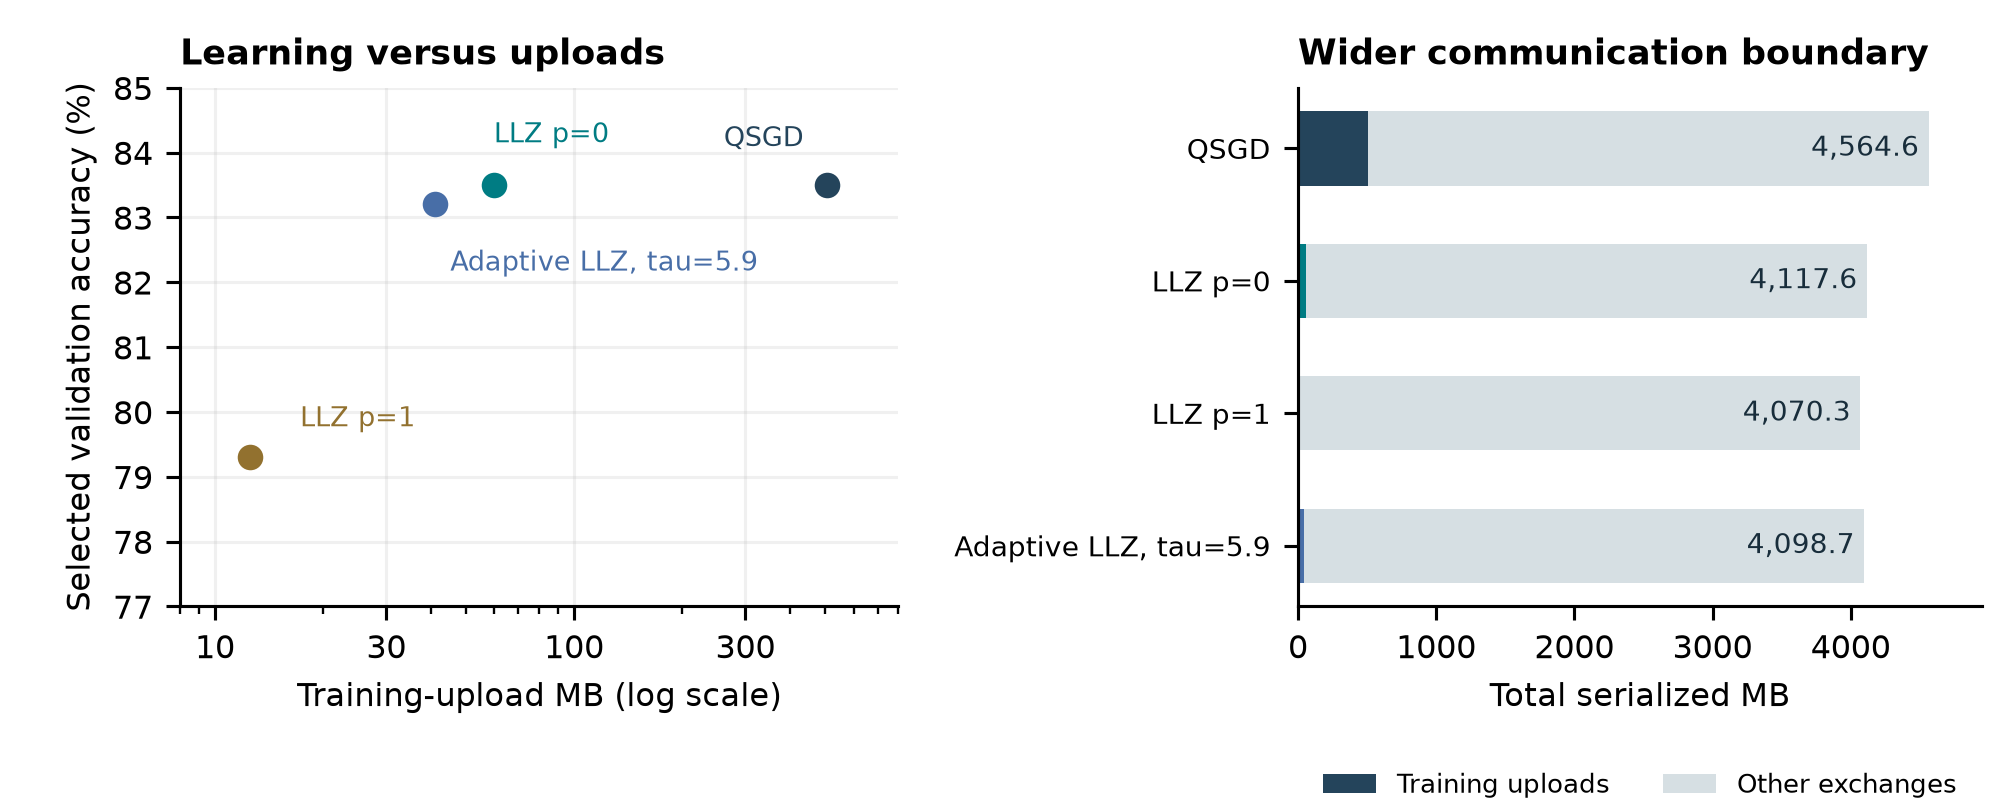
\includegraphics[width=0.97\textwidth]{figures/pilot-communication.png}
\caption{Completed WSL DigiFace seed-42 development batch. Left: selected validation accuracy versus training-upload MB (log x-axis). Right: serialized Flower-object totals split into training uploads and all other exchanges. No error bars are inferred from one seed; test-set evaluation was disabled.}
\label{fig:pilot}
\end{figure}

Training-upload savings versus QSGD were 88.20\% for p=0, 97.54\% for p=1 and 91.93\% for adaptive LLZ (tau=5.9). Best validation accuracies were 83.5\%, 79.3\% and 83.2\%, respectively, against 83.5\% for QSGD. Adaptive LLZ passed the predeclared 1.0-point single-seed gate; this is not evidence of statistical equivalence.

Total serialized-object savings were 9.8\%, 10.8\% and 10.2\%; these Flower object bytes are not network traffic. Across 60 adaptive client-round records, selected p counts were 0: 35, 1: 18 and 2: 7; maximum additional-error ratio was 5.895 under the 5.9 limit. For p=0, all 15 model hashes, validation records and shared QSGD metrics matched, with zero LLZ reconstruction error. The baseline source differed only in the p=0 parser and timeout allowance; numerical replay matched, source hashes did not.

This is one-seed evidence; controlled timing, budget sensitivity and confirmation remain.

\section{Interpretation, reproducibility and next evidence}

A useful review conclusion is that compression quality has at least three axes: learning behavior, complete communication and computational cost. A codec-correct adaptive selector is one component of the research framework, rather than evidence that the learning-safe budget has been solved. Our pilot demonstrates that an upload saving can nearly disappear at a wider communication boundary and that a looser reconstruction budget need not improve the accuracy/byte trade-off.

\begin{table}[htbp]
\centering
\small
\begin{tabularx}{\textwidth}{R{0.98000}R{1.02000}}
\toprule
\textbf{Established in this review} & \textbf{Still open / not established} \\\midrule
p=0 replay and saved pilot accounting & Learning-safe budget or statistical equivalence \\
\rowcolor{TableAlt}
Finite feasible selector and complete-reply costs & Optimal aggregate traffic across changing trajectories \\
Published compression/EF precedents & A theorem for our actual no-EF local epochs \\
\rowcolor{TableAlt}
AE offline feasibility evidence & AE identification accuracy in FL \\
Seven-candidate recent search & An exhaustive novelty or priority conclusion \\
\bottomrule
\end{tabularx}
\caption{Evidence boundaries for the thesis. Proposed extensions are not relabeled as completed results.}
\label{tab:evidence}
\end{table}

\subsection*{How the pilot results are obtained}

The reproducible evidence chain is: frozen protocol and source/data fingerprints; training-only saved updates for initial calibration; matched initialization and data/model settings; client-local training deltas; one QSGD draw and encoded LLZ candidates; locally decoded error/byte measurements; selected reply and server reconstruction; per-round validation and communication ledgers; validation-loss checkpoint selection; saved comparison summary. This review's plot and table are generated from that final JSON summary, not manually transcribed chart points.

Tau=5.9 was carried forward from a training-only calibration heuristic, not selected by a convergence theorem or validation outcome; the run's maximum observed ratio sits close to its boundary. The exact rationale and sensitivity to other budgets remain open, and seed 43/44 confirmation is not yet available. The earlier manuscript and the IEEE publication are kept as different provenance records rather than retroactively relabeling the implementation source. \parencite{cao2026llzmanuscript,cao2026llz}

\subsection*{Research direction}

The immediate priority is a transparent budget-sensitivity study followed by confirmation on new seeds, while holding the current dataset, model and local training fixed. Compare the observed bytes and additional error for candidate budgets, declare the learning-quality gate before confirmation, and report adaptive-search time. A matched EF ablation is a useful paper-inspired extension because the LLZ paper's empirical default differs from our pilot; it needs a specified residual protocol and compute budget. Full CIFAR/PowerSGD reproduction, LLZ-SI and additional model tuning are separate tasks.

The main research contribution can be a transparent LLZ-specific selector, complete byte/error/time accounting and defensible evidence about budget policies. A convergence theorem would require a derivation for the actual composed compressor and local-update algorithm. The present literature and pilot motivate that work; they do not replace it.
